The C2 and D2 observables were found to be very powerful to distinguish between one- and two-prong like jets, see e.g. Reference \cite{bib:power_counting}. They are defined as ratios of the so called \textit{Energy Correlation Functions} ECF(N,$\beta$) which explore the substructure of a jet using a sum over the constituents. These variables are IRC-safe ($\beta\ge0$) and theoretically well understood, see Reference \cite{bib:analytic_ECF}. D2 was found to perform slightly better for tagging $W$ jets as C2 in Reference \cite{bib:w_tagging}, most notably due to a more $p_{\mathrm{T}}$ robust cut value and somewhat higher background rejections. 
\begin{equation}
\begin{aligned}
 & \text{C2($\beta$)} ={} \frac{\text{ECF(3,$\beta$)}\cdot\text{ECF(1,$\beta$)}}{\text{ECF(2,$\beta$)}^2} \\ 
 & \text{D2($\beta$)} ={} \frac{\text{ECF(3,$\beta$)}\cdot\text{ECF(1,$\beta$)}^3}{\text{ECF(2,$\beta$)}^3}
\end{aligned}
\end{equation}\label{eq:C2D2} 
The constituents are correlated via a product of their $p_{\mathrm{T}}$, weighted by an angular factor. This factor is calculated from the pairwise angular distances of the considered constituents. An additional exponent $\beta$ scales this factor. The default value for $\beta$ is 1, corresponding to angular and momentum parts being weighted equally.
\begin{equation}
\begin{aligned}
 & \text{ECF(1)}  ={} \sum\limits_{constituents} p_{\mathrm{T}} \\ 
 & \text{ECF(2,$\beta$)} ={} \sum\limits_{i=1}^n \sum\limits_{j=i+1}^n p_{\mathrm{T},i}p_{\mathrm{T},j}\Delta R_{ij}^{\,\beta} \\ 
 & \text{ECF(3,$\beta$)} ={} \sum\limits_{i=1}^n \sum\limits_{j=i+1}^n \sum\limits_{k=j+1}^n p_{\mathrm{T},i}p_{\mathrm{T},j}p_{\mathrm{T},k}(\Delta R_{ij} \Delta R_{ik} \Delta R_{jk})^{\,\beta}
\end{aligned}
\end{equation}\label{eq:ECF}
ECF(2,$\beta$) uses pairwise correlation and is sensitive to two-prong structures. ECF(3,$\beta$) relies on triple-wise correlations to identify three-prong structures. ECF(1,$\beta$) corresponds to the $p_{\mathrm{T}}$ of the whole jet and serves as normalization to minimize the dependence on the energy scale.

For collinear or soft configurations of $N$ constituents, ECF(N,$\beta$) acquires very small values. Given ECF(2,$\beta$), only well angular separated and non-soft constituent pairs act as non-negligible sum terms. This directly leads to the picture of two hard substructures inside the jet. A similar conclusion can be done for ECF(3,$\beta$) and three hard substructures. 
A jet with $N$ or more hard substructures features a higher ECF(N, $\beta$) value as a jet consisting of fewer than $N$ prongs. Consequently, the ratios C2 and D2 can be used to separate these topologies.

A $W$ jet features a small ECF(3,$\beta$) but a high ECF(2,$\beta$) value resulting in small C2/D2, corresponding to a high agreement with the two-prong hypothesis. QCD jets feature a very small ECF(3,$\beta$) and a small ECF(2,$\beta$) value. Considering the power of ECF(2,$\beta$), this results in a higher C2/D2 value as for a $W$ jet. A $W$ tagging example for C2 and D2 with clusters as input is given in Figure \ref{fig:ECF_example}.
\begin{figure}
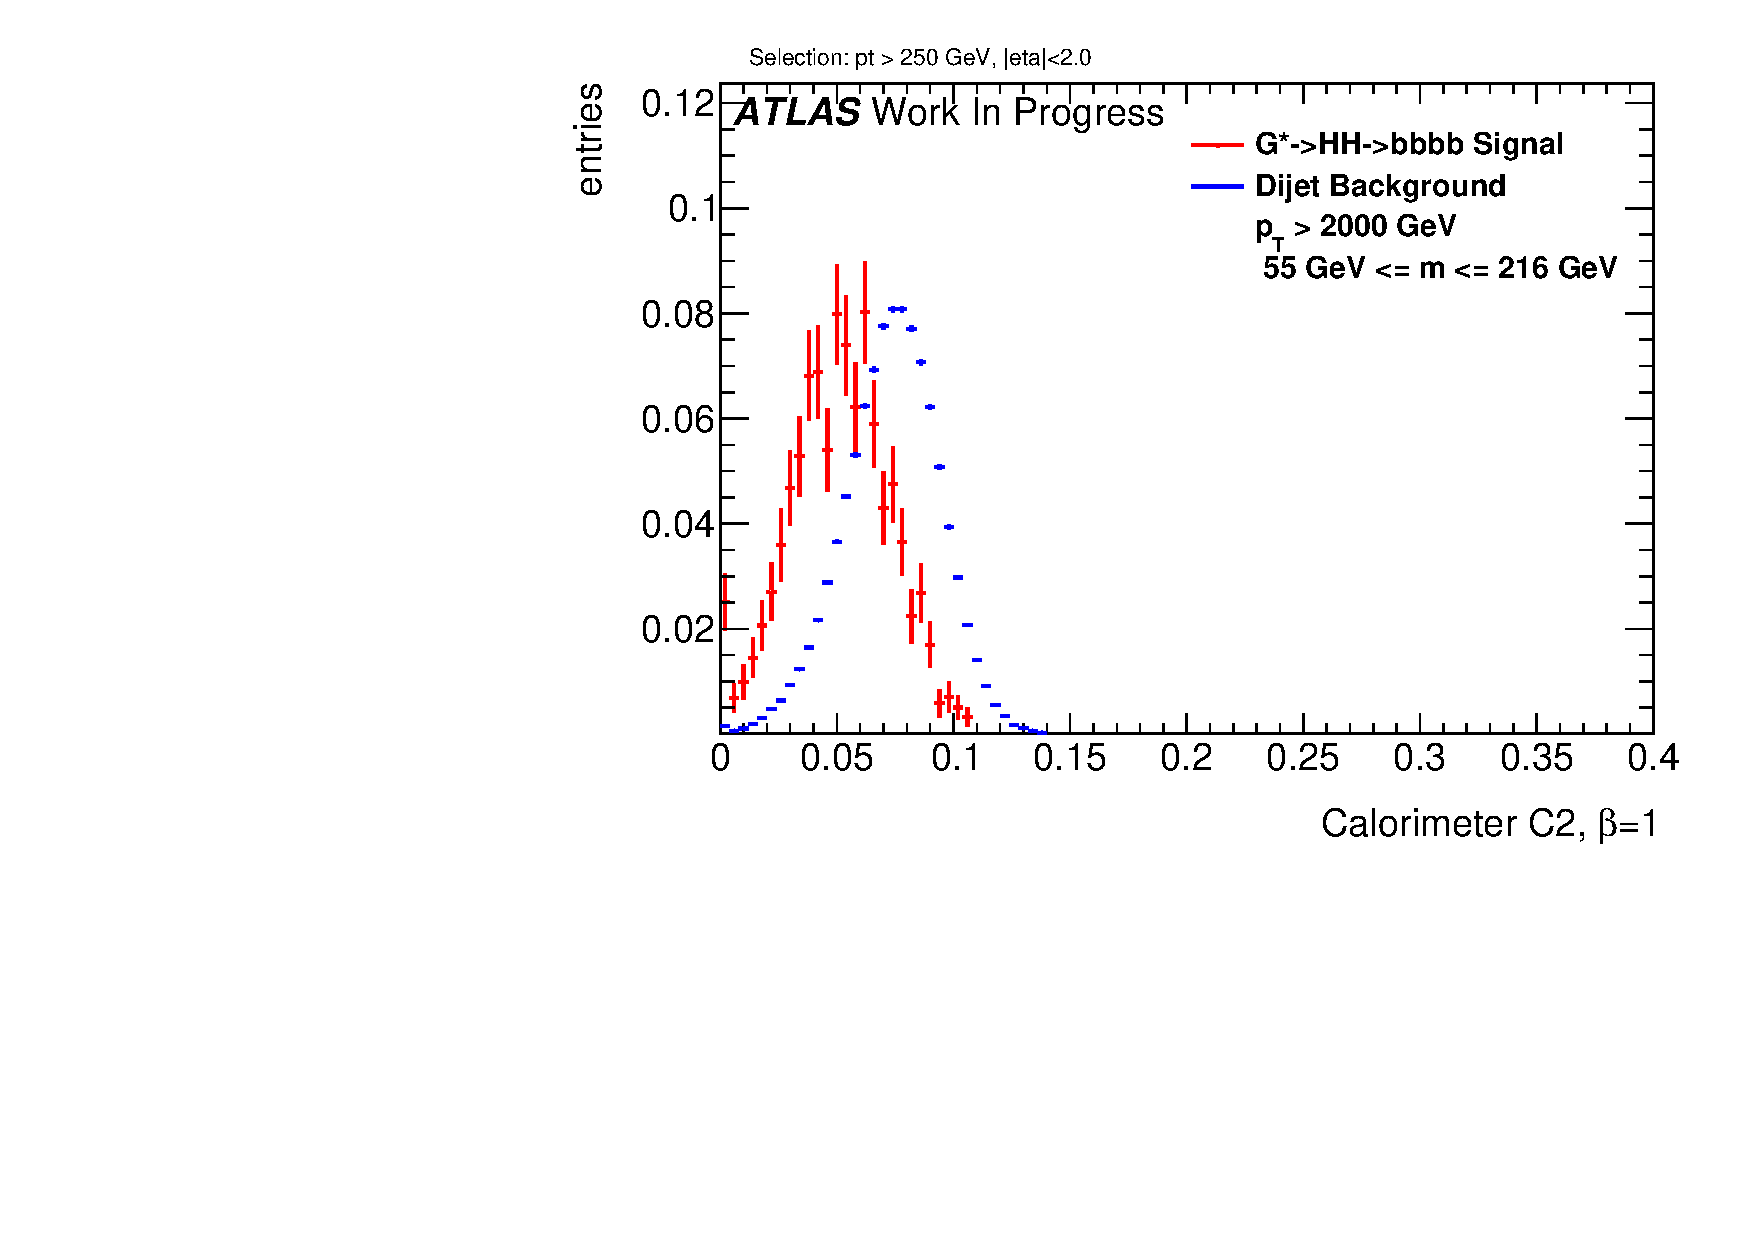
\includegraphics[width=0.5\textwidth]{sascha_input/plots/W/Beta1/h_recoJet_C2_bin6.pdf} \hspace{1mm}
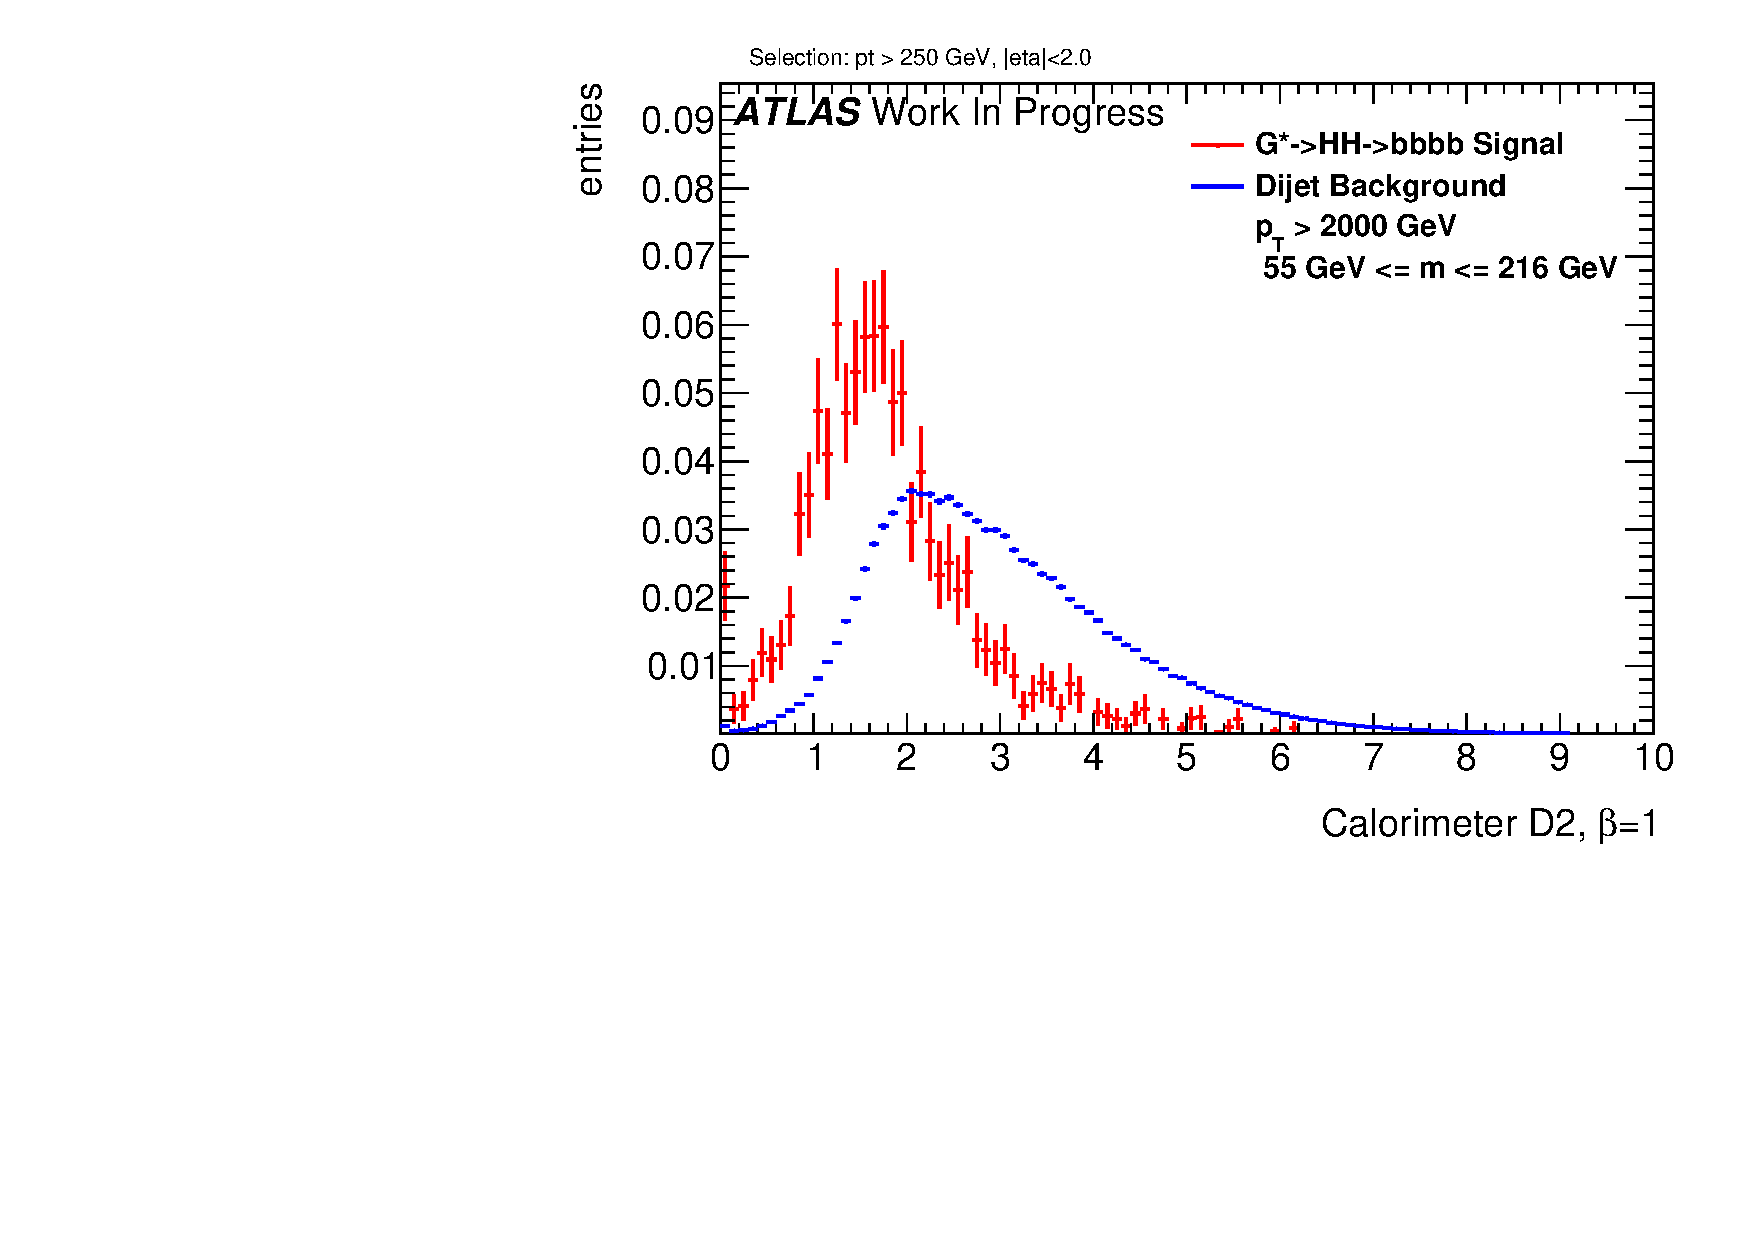
\includegraphics[width=0.5\textwidth]{sascha_input/plots/W/Beta1/h_recoJet_D2_bin6.pdf} 
\caption{Exemplary C2 (left) and D2 (right) distributions for $W$ signal jets and QCD background jets, calculated with clusters. In both cases the background tends to higher values.}\label{fig:ECF_example}
\end{figure}